\documentclass[a4paper, twocolumn]{ltjsarticle}

% 画像
\usepackage[dvipdfmx]{graphicx}
% 表
\usepackage{booktabs}
\usepackage{enumerate}

% 数式
\usepackage{amsmath}
\usepackage{amssymb}
\usepackage{amsfonts}

% ベクトル
\usepackage{bm}
% コード
\usepackage{listings,jvlisting}
% コードの色
\usepackage{color}
\usepackage{subcaption}
\usepackage{array}

\definecolor{OliveGreen}{rgb}{0.0,0.6,0.0}
\definecolor{Orenge}{rgb}{0.89,0.55,0}
\definecolor{SkyBlue}{rgb}{0.28,0.28,0.95}
% ここからコードの表示に関する設定
\lstset{
  language=C++,
  basicstyle={\ttfamily},
  identifierstyle={\small},
  commentstyle={\small\itshape},
  keywordstyle={\small\bfseries},
  ndkeywordstyle={\small},
  stringstyle={\small\ttfamily},
  frame={tb},
  breaklines=true,
  columns=[l]{fullflexible},
  numbers=left,
  xrightmargin=0zw,
  xleftmargin=3zw,
  numberstyle={\scriptsize},
  stepnumber=1,
  numbersep=1zw,
  lineskip=-0.5ex,
  keepspaces=true,
  keywordstyle={\color{SkyBlue}},
  commentstyle={\color{OliveGreen}},
  stringstyle=\color{Orenge},
  showstringspaces=false
}
\renewcommand{\lstlistingname}{Code}
\newcommand{\E}[1]{\times10^{#1}}



\title{人工知能 中間レポート 課題4}
\author{03420414  小松麟太郎}
\date{\today}


\begin{document}

\maketitle

\subsection*{問題1}
図1のナイトツアーの解を幅優先探索，深さ優先探索，A*探索を用いて探索した．深さ優先探索の反復深化のための定数 $D$ は 6 とした．また，A*探索の評価関数 $f(n)$ としては以下の関数 $f(n)$ を用いた．
\begin{equation}
    f_1(n) = d(n) + h(n)
\end{equation}
ただし，$d(n)$ はノードの深さ，$h(n)$ は目標状態と異なる位置にある数字の数である．それぞれのアルゴリズムを用いた場合の，子ノードの数，解の長さは表1のようになった．いずれのアルゴリズムも長さ5の解を見つけた．子ノードの数は A* 探索が1番少なく，5つだけだった．次に子ノードの数が多いのが幅優先探索で 7 個，そして1番多かったのが深さ優先探索で11個だった．
\begin{figure}[ht]
    \centering
    \begin{minipage}{0.45\linewidth}
        \flushright
        \begin{tabular}{|c|c|c|}
            \hline
            8 & 2 & 4 \\ \hline
            9 & 5 & 6 \\ \hline
            7 & 3 & 1 \\ \hline
        \end{tabular}

        \subcaptionsetup{justification=raggedleft, singlelinecheck=false }
        \subcaption{初期状態}
    \end{minipage}
    \hfill
    \begin{minipage}{0.45\linewidth}
        \flushleft
        \begin{tabular}{|c|c|c|}
            \hline
            1 & 2 & 3 \\ \hline
            4 & 5 & 6 \\ \hline
            7 & 8 & 9 \\ \hline
        \end{tabular}

        \subcaptionsetup{justification=raggedright, singlelinecheck=false }
        \subcaption{ 目標状態}
    \end{minipage}
    \caption{}
\end{figure}
\begin{table}[h]
    \centering
    \begin{tabular}{@{}c|cc@{}}
        \hline
        & 子ノードの数 & 解の長さ\\
        \hline
        幅優先探索 & 7 & 5 \\ 
        深さ優先探索 & 11 & 5 \\ 
        A*探索 & 5 & 5 \\ 
        \hline
    \end{tabular}
    \caption{問題1の結果}
\end{table}
\subsection*{問題2}
図2のナイトツアーの解を幅優先探索，深さ優先探索，A*サーチを用いて探索した．各アルゴリズムの条件は問題1と同じとした．それぞれのアルゴリズムを用いた場合の，子ノードの数，解の長さは表2のようになった．いずれのアルゴリズムも長さ12の解を見つけた．子ノードの数は A* 探索が1番少なく，52個だった．一方で，幅優先探索と深さ優先探索の場合は子ノードの数がそれぞれ，4786個と1743個であり，A*探索の52個より30～100倍ほどになっており，A*探索がほかの2つの方法より有効であることが分かる．
\begin{figure}[ht]
    \centering
    \begin{minipage}{0.45\linewidth}
        \centering
        \begin{tabular}{|@{\hskip 3.5pt}c@{\hskip 3.5pt}|@{\hskip 3.5pt}c@{\hskip 3.5pt}|@{\hskip 3.5pt}c@{\hskip 3.5pt}|@{\hskip 3.5pt}c@{\hskip 3.5pt}|}
            \hline
            10 & 1 & 12 & 4\\ \hline
            5 & 13 & 7 & 9\\ \hline
            15 & 3 & 2 & 6\\ \hline
            11 & 14 & 8 & 16\\ \hline
        \end{tabular}
        \subcaption{初期状態}
    \end{minipage}
    \hfill
    \begin{minipage}{0.45\linewidth}
        \centering
        \begin{tabular}{|@{\hskip 3.5pt}c@{\hskip 3.5pt}|@{\hskip 3.5pt}c@{\hskip 3.5pt}|@{\hskip 3.5pt}c@{\hskip 3.5pt}|@{\hskip 3.5pt}c@{\hskip 3.5pt}|}
            \hline
            1 & 2 & 3 & 4\\ \hline
            5 & 6 & 7 & 8\\ \hline
            9 & 10 & 11 & 12\\ \hline
            13 & 14 & 15 & 16\\ \hline
        \end{tabular}
        \subcaption{ 目標状態}
    \end{minipage}
    \caption{}
\end{figure}
\begin{table}[h]
    \centering
    \begin{tabular}{@{}c|cc@{}}
        \hline
        & 子ノードの数 & 解の長さ\\
        \hline
        幅優先探索 & 4786 & 12 \\ 
        深さ優先探索 & 1743 & 12 \\ 
        A*探索 & 52 & 12 \\ 
        \hline
    \end{tabular}
    \caption{問題2の結果}
\end{table}
\newpage
\subsection*{問題3}
図3のナイトツアーの解を幅優先探索，深さ優先探索，A*サーチを用いて探索した．この問題では，最初の操作では1を動かすが，その後はある一定の回数 $L$ 同じ数字を動かした後には動かす数字を切り替えてもよいというルールを追加した．例えば，$L = 5$ のとき，まず 1 を 5回動かし，そのあとに 7を8回動かし，8を5回動かすというような操作ができる．
\begin{figure}[h]
    \centering
    \begin{minipage}{0.45\linewidth}
        \centering
        \begin{tabular}{|@{\hskip 3.5pt}c@{\hskip 3.5pt}|@{\hskip 3.5pt}c@{\hskip 3.5pt}|@{\hskip 5pt}c@{\hskip 5pt}|@{\hskip 5pt}c@{\hskip 5pt}|}
            \hline
            16 & 12 & 8 & 4\\ \hline
            15 & 11 & 7 & 3\\ \hline
            14 & 10 & 6 & 2\\ \hline
            13 & 9 & 5 & 1\\ \hline
        \end{tabular}
        \subcaption{初期状態}
    \end{minipage}
    \hfill
    \begin{minipage}{0.45\linewidth}
        \centering
        \begin{tabular}{|@{\hskip 3.5pt}c@{\hskip 3.5pt}|@{\hskip 3.5pt}c@{\hskip 3.5pt}|@{\hskip 3.5pt}c@{\hskip 3.5pt}|@{\hskip 3.5pt}c@{\hskip 3.5pt}|}
            \hline
            1 & 2 & 3 & 4\\ \hline
            5 & 6 & 7 & 8\\ \hline
            9 & 10 & 11 & 12\\ \hline
            13 & 14 & 15 & 16\\ \hline
        \end{tabular}
        \subcaption{ 目標状態}
    \end{minipage}
    \caption{}
\end{figure}
\\\quad $L$ の値を変えながら，問題1と同じ，幅優先探索，深さ優先探索，A*サーチを実行したが，どの方法でも子ノードの数が800万から1500万ほどになったところで，メモリの上限に達したのかプロセスがkillされてしまい，解を見つけることができなかった．そこで A* 探索の評価関数について次の $f_2(n)$, $f_3(n)$ を考えた．
\begin{align}
    f_2(n) &= d(n) + h(n) + p_1(n)\\
    f_3(n) &= d(n) + h(n) + p_2(n)
\end{align}
ただし，$p_1(n)$ は各数字の目標状態とのマンハッタン距離の和，$p_2(n)$ は各数字の目標状態とのマンハッタン距離を3で割った余りの和である．$p_2(n)$ でマンハッタン距離を3で割った余りをとったのは，ナイトを動かすとマンハッタン距離は3ずつ変わるので，目標状態とのマンハッタン距離が3の倍数であるものの方が目標状態に近づきやすいと考えらからである．\\
\begin{figure}[b]
    \centering
    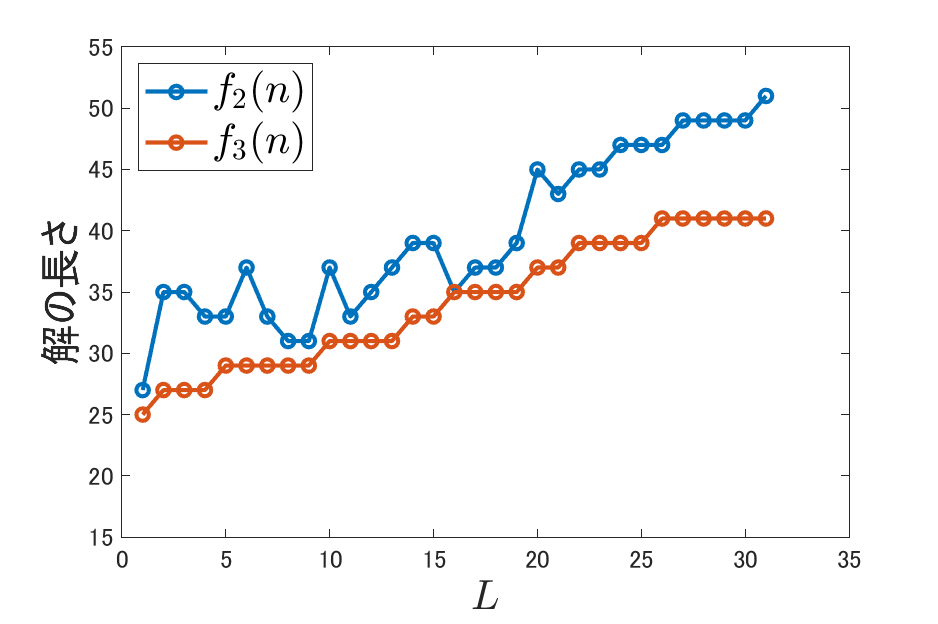
\includegraphics[width=\linewidth]{answer_length.png}
    \caption{解の長さ}
\end{figure}
\begin{figure}[b]
    \centering
    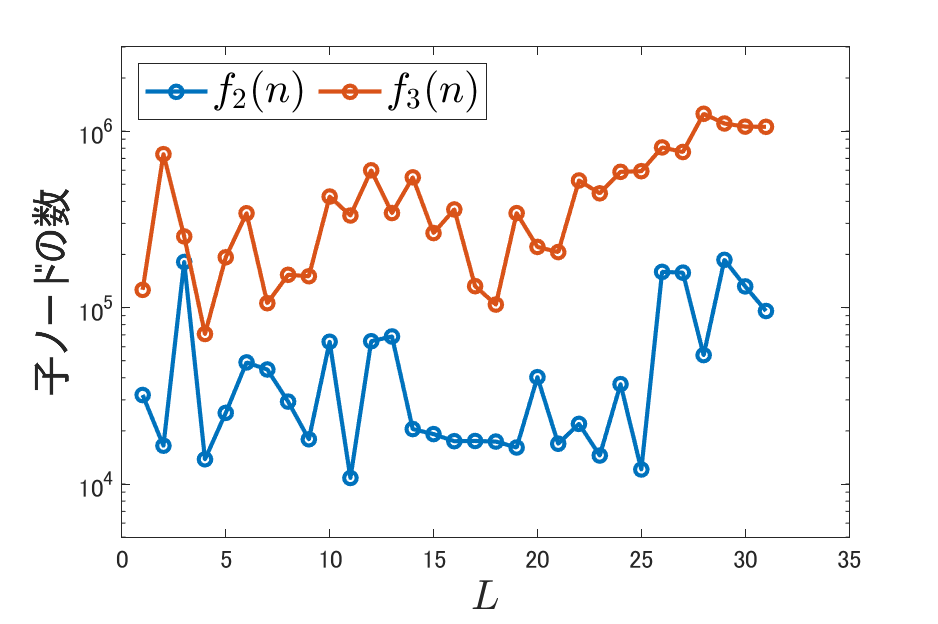
\includegraphics[width=\linewidth]{numchild.png}
    \caption{子ノードの数}
\end{figure}
\quad この $f_2(n)$, $f_3(n)$ を評価関数として A* 探索を実行すると解を見つけることができた．次の図4，5 はそれぞれ $L$ の値を変えたときの解の長さと子ノードの数をグラフで表したものである．評価関数として $f_2(n)$ を用いたときには，$L = 1$ としたときに見つけた長さ 27 の解が一番短いもので，子ノードの数は $L$ の値によって，$10^4$ から $2\E{5}$ の間で変動した．$f_3(n)$ を評価関数として用いたときには，$L = 1$ としたときに見つけた長さ 25  の解が一番短いもので， $f_2(n)$ が見つけたのもより短い解を見つけることができた．また, どの $L$ でも $f_3(n)$ が見つけた解は $f_2(n)$ が見つけた解よりも短かった． 一方で，子ノードの数は $7\E{4}$ から $1.3\E{6}$の間で変動しており，$f_2(n)$ の約 10 倍になった．このことから，$f_2(n)$ は少ないノード数で解を見つけるのが優れており，$f_3(n)$ は短い解を見つけるのに優れていることが分かる．どちらの場合も，$L$ の値を大きくすると解の長さは大きくなっていった．これは，$L$ の長さが大きいと動かす数字の柔軟性が小さくなるので，解の長さが小さくなるのは自然なことだと考えられる．一方 $L$ を小さくしても，柔軟性が増すことで，子ノードの数が急激に増加することはなかった．したがって，最適な解を見つける場合は $L = 1$ とするのがいいと考えられる．


\begin{figure}[b]
    \centering
    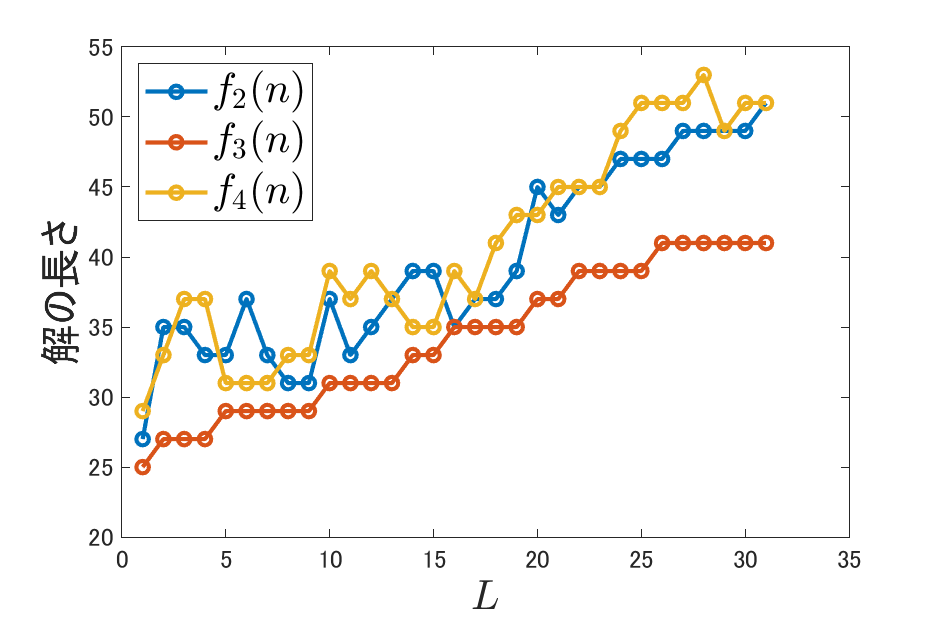
\includegraphics[width=\linewidth]{answer_length1.png}
    \caption{解の長さ}
\end{figure}
\begin{figure}[b]
    \centering
    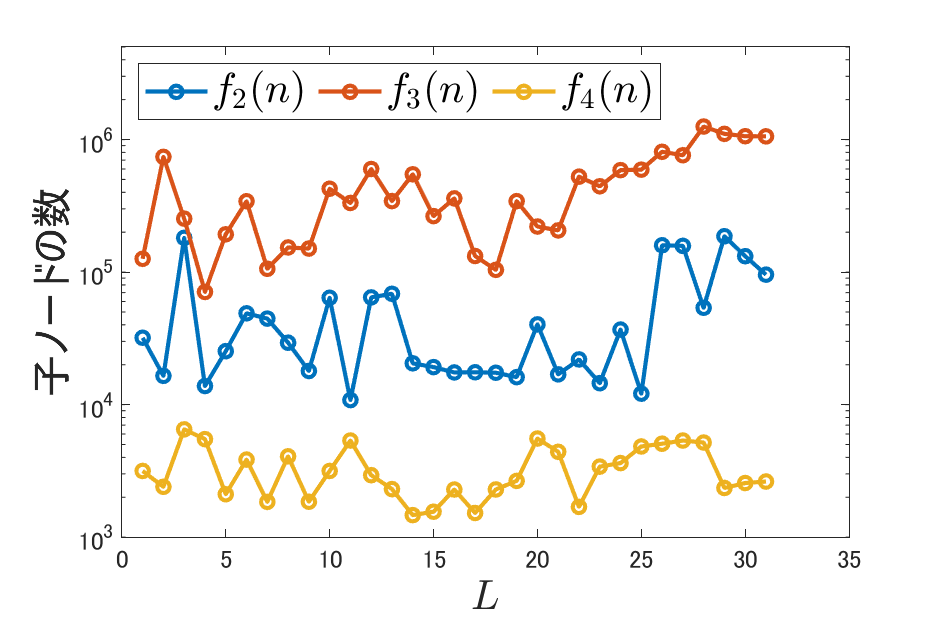
\includegraphics[width=\linewidth]{numchild1.png}
    \caption{子ノードの数}
\end{figure}
評価関数として， $f_2(n)$, $f_3(n)$ から，$h(n)$ を抜いたもの，つまり目標状態とのマンハッタン距離とノードの深さのみを考えたものを用いても，解を見つけることができなかったが．$h(n)$ を加えることで解を見つけることができた．このことから，評価関数を複雑化することによって，解が見つけやすくなる良い評価関数にことがあるということが予想される．\\
\quad そこで， $f_2(n)$, $f_3(n)$ を組み合わせた次の評価関数 $f_4(n)$ を考えた．
\begin{equation}
    f_4(n) = d(n) + h(n) + p_1(n) +p_2(n)
\end{equation}
次の図6，7 はそれぞれ $L$ の値を変えたときの解の長さと子ノードの数をグラフで表したものである．解の長さは $L = 1$ のときに一番短くなり，長さ29の解を見つけた．ほかの $L$ の場合でも $f_2(n)$ とあまり変わらず，$f_3(n)$ を用いた場合よりも短い解を見つけることはできなかった．一方で，子ノードの数は $10^3$ から $10^4$ の間で変動し，$f_2(n)$ の約 10 分の1，$f_3(n)$ の約 100 分の1 ほどになり，より少ないノード数で解を見つけることができた． $f_2(n)$, $f_3(n)$ を組み合わせることによって，より早く解を見つけることができたが，より短い解を見つけることができるのはマンハッタン距離を3で割った余りを考える，$f_3(n)$ であることが分かった．
\end{document}
